\section{Offline RL}
\label{sec:offlineRL}

\begin{figure}
\centering
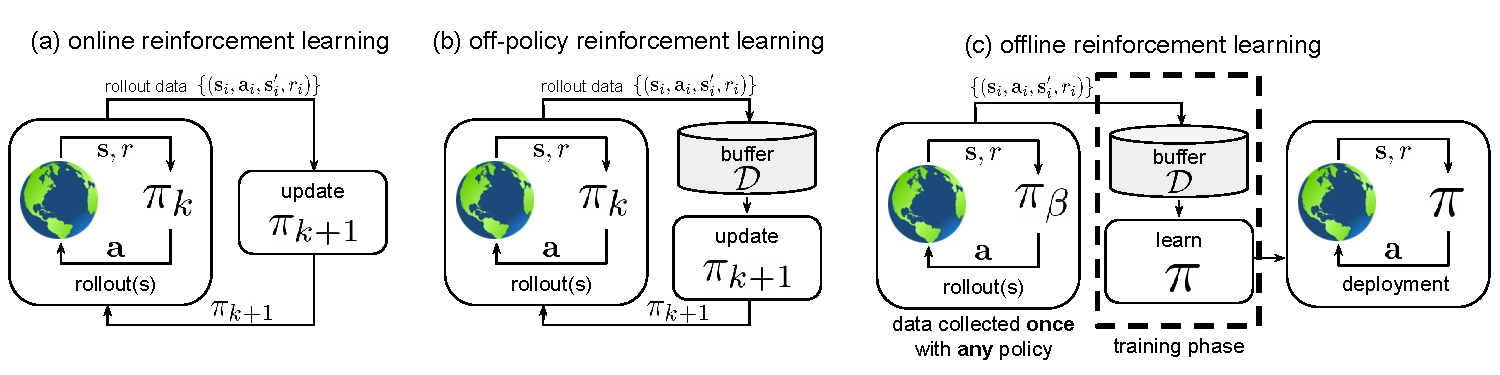
\includegraphics[height=1.5in]{figs/offlineRL}
\caption{
  Comparison of online on-policy RL,  online off-policy RL,
  and offline RL.
\figtaken{Figure 1 of \citep{Levine2020offline}}.
\figthanks{Sergey Levine}.
}
\label{fig:offline}
\end{figure}




\keywordDef{Offline reinforcement learning}
(also called \keywordDef{batch reinforcement learning} \cite{Lange2012})
is concerned with learning a reward maximizing
policy from a fixed, static dataset,
collected by some existing policy,
known as the \keywordDef{behavior policy}.
Thus no interaction with the environment is allowed
(see \cref{fig:offline}).
This makes policy learning harder than the online case,
since we do not know the consequences of actions that were not taken
in a given state, and cannot test any such ``counterfactual'' predictions
by trying them.
(This is the same problem as in off-policy RL, which we discussed in
\cref{sec:offpolicy}.)
In addition, the policy will be deployed on new states that it may not have seen,
requiring that the policy generalize out-of-distribution,
which is the main bottleneck for current offline RL methods \citep{Park2024value}.
%We discuss some solution methods below.
%(See also \citep{Bhargava2024} for a recent comparison
%of the methods we will discuss.)

A very simple and widely used offline RL method
is known as \keyword{behavior cloning} or \keyword{BC}.
This amounts to training a policy to predict the observed
output action $a_t$ associated with each observed state $s_t$,
so we aim to ensure $\pi(s_t) \approx a_t$,
as in supervised learning.
This assumes the offline dataset was created by an expert,
and so falls under the umbrella of imitation learning
(see \cref{sec:BC} for details).
By contrast, offline RL methods can leverage suboptimal data.
We give a brief summary of some of these  methods below.
For more details, 
see e.g., \citep{Levine20Offline,Chen2024offlineRL,Cetin2024}.
For some offline RL benchmarks,
see DR4L \citep{Fu20}, RL Unplugged \citep{Gulcehre20},
OGBench (Offline Goal-Conditioned benchmark) \citep{Park2024},
and D5RL \citep{Rafailov2024}.

%A simple extension of BC to the case where
%the offline dataset was generated by policies of variable
%quality is to filter out trajectories with low reward;
%this is called \keywordDef{filtered BC}.




%For an experimental comparison of
%offline RL methods, see e.g., \citep{Gulcehre20,Fu20,Bhargava2024,Cetin2024}.
%For a more recent approach,
%known as \keywordDef{perceiver actor critic},
%see \citep{Springenberg2024}.


\subsection{Offline model-free RL}


In principle, we can tackle offline RL using the off-policy methods
that we discussed in \cref{sec:offpolicy}.
These use some form of importance sampling, based on
$\policytgt(a|s)/\behavior(a|s)$, to reweight the data in the replay buffer $\data$,
which was collected by 
the behavior policy, towards the current policy (the one  being evaluated/ learned).
Unfortunately, such methods only work well if the behavior policy is
is close to the new policy. In the online RL case,
this can be ensured by gradually updating the new policy away from
the behavior policy, and then sampling new data  
from the updated policy (which becomes the new behavior policy).
Unfortunately, this is not an option in the offline case.
Thus we need to use other strategies to control the discrepancy
between the behavior policy and learned policy, as we discuss below.
(Besides the algorithmic techniques we discuss,
another reliable way to get better offline RL performance
is to train on larger, more diverse datasets,
as shown in \citep{Kumar2023offline}.)

\eat{
Various methods have been developed to control the variance
of the importance weights in the offline case,
as discussed in \citep[Sec 4]{Levine20Offline},
but such methods are not widely used in practice.
}

\subsubsection{Policy constraint methods}

In the \keywordDef{policy constraint} method,
we use a modified form of  actor-critic,  which, at iteration $k$,
uses an update of the form
\begin{align}
  Q^{\pi}_{k+1} &\leftarrow \argmin_Q \expectQ{
    \left(Q(s,a) - (R(s,a) + \gamma \expectQ{Q^{\pi}_k(s',a')}{\pi_k(a'|s')})
    \right)^2
  }{(s,a,s') \sim \data} \\
  \pi_{k+1} &\leftarrow \argmax_{\pi} \expectQ{
    \expectQ{Q^{\pi}_{k+1}(s,a)}{\pi(a|s)}}{s \sim \data}
  \myst D(\policy, \behavior) \leq \epsilon
  \label{eqn:piUpdate}
\end{align}
where $D(\policy(\cdot|s), \behavior(\cdot|s))$ is a divergence measure
on distributions, such as KL divergence or another $f$-divergence.
This ensures that we do not try to evaluate the $Q$ function
on actions $a'$ that are too dissimilar from those seen
in the data buffer (for each sampled state $s$),
which might otherwise result in artefacts similar
an  adversarial attack.


As an alternative to adding a constraint,
we can add a penalty of
$\alpha D(\policy(\cdot|s), \behavior(\cdot|s))$
to the target $Q$ value and the actor objective,
resulting in the following update:
\begin{align}
  Q^{\pi}_{k+1} &\leftarrow \argmin_Q \expectQ{
    \left(Q(s,a) - (R(s,a) + \gamma \expectQ{Q^{\pi}_k(s',a')
    -\alpha \gamma D(\pi_k(\cdot|s'), \behavior(\cdot|s'))}{\pi_k(a'|s')})
    \right)^2
  }{(s,a,s') \sim \data} \\
  \pi_{k+1} &\leftarrow \argmax_{\pi} \expectQ{
    \expectQ{Q^{\pi}_{k+1}(s,a)}{\pi(a|s)}
  - \alpha D(\pi(\cdot|s'), \behavior(\cdot|s'))}{s \sim \data}
\end{align}

One problem with the above method is that we have to fit
a parametric model to $\behavior(a|s)$ in order to evaluate the
divergence term. Fortunately, in the case of KL, the divergence
can be enforced implicitly,
as in the \keywordDef{advantage weighted regression}
or \keywordDef{AWR} method of \citep{Peng2019awr},
the \keywordDef{reward weighted regression} method
of \citep{Peters07},
 the \keywordDef{advantage weighted actor critic}
or \keywordDef{AWAC} method of \citep{Nair2020},
the \keywordDef{advantage weighted behavior model}
or \keywordDef{ABM} method of \citep{Siegel2020},
In this approach, we first solve (nonparametrically) for the new policy
under the KL divergence constraint to
get $\overline{\pi}_{k+1}$, and then we project
this into the required policy function class via
supervised regression, as follows:
\begin{align}
  \overline{\pi}_{k+1}(a|s) &\leftarrow \frac{1}{Z}
  \behavior(a|s) \exp\left( \frac{1}{\alpha} Q_k^{\pi}(s,a) \right) \\
  \pi_{k+1} &\leftarrow \argmin_{\pi} \KLpq{\overline{\pi}_{k+1}}{\pi}
\end{align}
In practice the first step can be implemented by weighting
samples from $\behavior(a|s)$ (i.e., from the data buffer)
using importance weights given by
$\exp\left( \frac{1}{\alpha} Q_k^{\pi}(s,a) \right)$,
and the second step can be implemented via  supervised
learning (i.e., maximum likelihood estimation) using
these weights.

It is also possible to replace the KL divergence
with an integral probability metric (IPM),
such as the maximum mean discrepancy (MMD) distance,
which can be computed from samples,
without needing to fit a distribution $\behavior(a|s)$.
This approach is used in 
\citep{Kumar2019off}.
% https://bair.berkeley.edu/blog/2019/12/05/bear/
This has the advantage that it can constrain the support of the learned
policy to be a subset of the behavior policy,
rather than just remaining close to it.
To see why this can be advantageous, consider the case where
the behavior policy is uniform.
In this case, constraining the learned policy to remain close (in KL divergence)
to this distribution could result in suboptimal behavior,
since the optimal policy may just want to put all its mass on a single action
(for each state).

\subsubsection{Behavior-constrained policy gradient methods}

Recently a class of methods has been developed that is simple and effective:
we first learn a baseline policy $\pi(a|s)$ (using BC) and a Q function
(using Bellman minimization) on the offline data,
and then update the policy parameters to pick actions that have high expected
value according to $Q$ and which are also likely under the BC prior.
%which we call behavior-regularized PG \citep{Wu2020}.
An early example of this is the $Q^{\dagger}$ algorithm
of \citep{Fujimoto2019batch}.
In  \citep{Fujimoto2021}, they present
 the \keywordDef{DDPG+BC} method,
which optimizes
\be
\max_{\pi} J(\pi) = \expectQ{
  Q(s,\mu^{\pi}(s)) + \alpha \log \pi(a|s)}{(s,a) \sim \data}
\ee
where $\mu^{\pi}(s) = \expectQ{a}{\pi(a|s)}$ is the mean of
the predicted action, and $\alpha$ is a hyper-parameter.
As another example,
the \keywordDef{DQL} method of \citep{Wang2023DQL}
optimizes a diffusion policy using
\be
\min_{\pi} \loss(\pi)
= \loss_{\text{diffusion}}(\pi) + \loss_{q}(\pi)
= \loss_{\text{diffusion}}(\pi) 
- \alpha \expectQ{Q(s,a)}{s \sim  \data,
  a \sim \pi(\cdot|s)}
\ee
Finally, \citep{Agarwal2022} discusses how to transfer
the policy from a previous agent to a new agent
by combining BC with Q learning.

\subsubsection{Uncertainty penalties}
\label{sec:offlineUncertainty}

An alternative way to avoid picking out-of-distribution actions,
where the $Q$ function might be unreliable,
is to add a penalty term to the $Q$ function based on the estimated
epistemic uncertainty, given the dataset $\data$,
which we denote by $\text{Unc}(P_D(Q^{\pi}))$,
where $P_D(Q^{\pi})$ is the distribution over $Q$ functions,
and $\text{Unc}$ is some metric on distributions.
For example, we can use a deep ensemble to represent the distribution,
and use the variance of $Q(s,a)$ across ensemble members as
a measure of uncertainty.
%as in \citep{Kumar2019off}.
This gives rise to the following policy improvement update:
\begin{align}
  \pi_{k+1} &\leftarrow \argmax_{\pi} \expectQ{
    \expectQ{
      \expectQ{Q^{\pi}_{k+1}(s,a)}{P_D(Q_{k+1}^{\pi})}
    }{\pi(a|s)}
    - \alpha \text{Unc}(P_D(Q_{k+1}^{\pi}))
}{s \sim \data}
\end{align}
For examples of this approach, see e.g.,
\citep{An2021,Wu2021unc,Ghasemipour2022}.

\subsubsection{Conservative Q-learning and pessimistic value functions}
\label{sec:CQL}
% Sergey Levine talk 2024
% https://www.youtube.com/watch?v=Az5BoT7lCYo&list=PLEA9Mnr-L18lI_I-EkyAc1-gXgBj52oV5


An alternative to explicitly estimating uncertainty
is to add a \keywordDef{conservative penalty}
directly to the $Q$-learning error term.
That is, we minimize the following wrt $\vw$
using each batch of data $\calB$:
\be
\overline{\calE}(\calB,\vw)
   = \alpha \calC(\calB,\vw) + \calE(\calB, \vw)
\ee
where $\calE(\calB, \vw) = \expectQ{ (Q_{\vw}(s,a) -
  (r+\gamma \max_{a'} Q_{\vw}(s',a')))^2}{(s,a,s') \in \calB}$
is the usual loss for $Q$-learning,
and $\calC(\calB,\vw)$ is some conservative penalty.
In the \keywordDef{conservative Q learning}
or \keywordDef{CQL} method of \citep{CQL},
we use the following penalty term:
\be
\calC(\calB,\vw)
= \expectQ{Q_{\vw}(s,a)}{s \sim \calB, a \sim \pi(\cdot|s)}
- \expectQ{Q_{\vw}(s,a)}{(s,a) \sim \calB}
\ee
If $\pi$ is the behavior policy, this penalty becomes 0.

 
\eat{
A natural approach to offline RL is to just perform
Q-learning on the fixed dataset,
and then to compute the policy using
$\pi(a|s) = \argmax_a Q(s,a)$.
In principle this should work, since Q-learning is off-policy,
but in practice it does not work.
The reason is that Q-learning is trying to learn
the optimal policy $\pi^*$, but the data was generated by
a fixed \keyword{behavior policy}
$\pi_{\beta}$, so when Q-learning predicts the value
of the best action, it cannot be checked against the data,
and it might become over optimistic.



To see this in more detail, let us rewrite
the Bellman backup in terms of a distribution
$\pi_{\tnew}$ that puts all its mass on the optimal action
(according to the current $Q$) for each state,
so $\pi_{\topt}(a|s)=\delta(a-\argmax_{a'} Q(s,a'))$.
Thus the TD loss becomes
\be
J_{\beta}(Q,\pi) = \expectQ{ (Q(s,a)-\targetV(s,a))^2}{\pi_{\beta}(s,a)}
\ee
where the target $\targetV(s,a)$ is defined by 
\be
\targetV(s,a) =
  r(s,a) + \expectQ{Q(s',a')}
  {\pi_{\beta}(s') \pi_{\topt}(a'|s')}
\ee
If we have $\pi_{\beta}(s,a)=\pi_{\beta}(s) \pi_{\topt}(s|a)$, this optimization
should work well, since the training data comes
from the optimal distribution, and thus we have a stable system.
But for suboptimal behavior data, Q-learning will learn
to find actions that do better than the training data,
according to $Q$; this is like finding adversarial examples
for a network, and can result in unstable behavior,
where the estimated $Q$ values increase, but the actual reward
decreases.

% Pessimism-based methods eg CQL
% Policy constraints (eg BRAC)
% Avoid OOD actions in updates (eg AWAC, IQL). Don't evaluate
%  actions you didn't train on.

One way to deal with the overestimation problem is to use
 \keywordDef{conservative Q learning}
 or \keywordDef{CQL} \citep{CQL}.
The idea is to find $(s,a)$ points where the
$Q$-function might be overestimating the true value,
and then to ``push down'' on the estimate,
so it becomes more conservative.
In practice this amounts to adding the following
regularizer (scaled by $\alpha$) to $J_{\beta}$:
\begin{align}
J_{CQL}(Q,\pi)
&=   \expectQ{ Q(s,a) -\expectQ{Q(s,a')}{a' \sim \pi(\cdot|s)}
}{(s,a) \sim \data} \\
&=  \expectQ{Q(s,a)}{(s,a) \sim \data}
- \expectQ{Q(s',a')}{s' \sim \data, a' \sim \pi(\cdot|s')}
\label{eqn:CQL}
\end{align}
%The first term in the regularizer pushes down on all
%$Q$ values, whereas the second term pushes up on
%the $Q$ values encountered in the data.
%One can prove that
%$\hat{Q}^{\pi} \leq Q^{\pi}$ for large enough $\alpha$.
%The $\alpha$ coefficient determines the strength of this
%regularization.


}

 \eat{
the approach attempts to generalize beyond  offline data,
but not too far.
First it uses Q learning to solve
\be
\argmin_{\vw} [Q_{\vw}(s_t,a_t) - \expectQ{r(s_t,a_t) + Q_{\vw}(s_{t+1},a_{t+1})}{\pemp}]^2
\ee
where $\pemp$ is the empirical distribution over trajectories.
It also fits the BC policy $q_{\beta}(a_t|s_t)$.
Finally  it finds the policy that is closest
(in the chosen parametric family)
to
$q(a_t|s_t) \propto \exp(Q_{\vw}(s_t,a_t) q_{\beta}(a_t|s_t))$,
which is the BC policy weigthed  by the Q function.
It does this by solving a weighted MLE problem
\be
\argmin_{\vtheta} \KLpq{\pi_{\vtheta}(a_t|s_t)}{q(a_t|s_t)}
\ee
%
 }


     
\subsection{Offline model-based RL}
\label{sec:offlineMBRL}


In \cref{sec:MBRL}, we discussed model-based RL,
which can train a dynamics model given a fixed dataset,
and then use this to generate synthetic data
to evaluate and then optimize  different possible policies.
However, if the model is wrong, the method may learn a suboptimal
policy, as we discussed in \cref{sec:modelUncertainty}.
This problem is particularly severe in the offline RL case,
since we cannot recover from any errors by collecting more data.
Therefore various conservative MBRL algorithms have been developed,
to avoid exploiting model errors.
For example, \citep{Kidambi2020} present the
\keywordDef{MOREL} algorithm,
and \citep{Yu2020mopo} present the \keywordDef{MOPO} algorithm.
Unlike the
value function uncertainty method of \cref{sec:offlineUncertainty},
or the conservative value function method of \cref{sec:CQL},
these model-based methods add a penalty for visiting states where
the model is likely to be incorrect.

In more detail, let $u(s,a)$ be an estimate of the uncertainty of the
model's predictions given input $(s,a)$.
In MOPO, they define a conservative reward using
$\overline{R}(s,a) = R(s,a) - \lambda u(s,a)$,
and in MOREL, they modify the MDP so that the agent enters an
absorbing state with a low reward when $u(s,a)$ is sufficiently
large.
In both cases, it is possible to prove that the model-based
estimate of the policy's performance under the modified
reward or dynamics is a lower bound of the performance
of the policy's true performance in the real MDP,
provided that the uncertainty function $u$ is an error oracle,
which means that is satisfies
$D(M_{\vtheta}(s'|s,a), M^*(s'|s,a)) \leq u(s,a)$,
where $M^*$ is the true dynamics, and $M_{\vtheta}$
is the estimated dynamics.

For more information on offline MBRL methods,
see \citep{Chen2024offline}.



 
\subsection{Offline RL using reward-conditioned sequence modeling}
\label{sec:seqModel}

Recently an approach to offline RL
based on sequence modeling has become very popular.
The basic idea --- known as \keywordDef{upside down RL}
\citep{Schmidhuber2019}
or \keywordDef{RvS} (RL via Supervised learning)
\citep{Kumar2019,Emmons2021} ---
is to train a generative model over future states
and/or actions conditioned on the observed reward,
rather than predicting the reward given a state-action
trajectory.
%This reduces to a supervised learning problem
%(albeit with high dimensional output).
At test time, the conditioning is changed
to represent the desired reward, and futures
are sampled from the model.
The implementation of this idea then depends on what
kind of generative model to use, as we discuss below.

The \keywordDef{trajectory transformer}
method of \citep{trajectoryTransformer}
learns a joint model of the form
$p(\vs_{1:T}, \va_{1:T}, \vr_{1:T})$
using a transformer,
and then samples from this using beam search,
selecting the ones with high reward (similar to MPC, \cref{sec:MPC}).
The \keywordDef{decision transformer} \citep{decisionTransformer}
is related, but  just generates action sequences,
and conditions on the past observations and the future reward-to-go.
That is, it fits
\be
\argmax_{\vtheta} \expectQ{
  \log \pi_{\vtheta}(a_t|s_{0:t}, a_{0:t-1}, \text{RTG}_{0:t})}{\pemp}
\ee
where $\text{RTG}_t = \sum_{k=t}^T r_t$ is the return to go.
(For a comparison of decision transformers to other offline RL methods,
see \citep{Bhargava2024}.)

The \keywordDef{diffuser} method of \citep{diffuser}
is a diffusion version of trajectory transformer,
so it fits $p(\vs_{1:T}, \va_{1:T}, \vr_{1:T})$ using diffusion,
where the action space is assumed to be continuous.
They also replace beam search with classifier guidance.
The \keywordDef{decision diffuser} method of \citep{decisionDiffuser}
extends diffuser by using classifer-free guidance,
where the conditioning signal is the reward-to-go,
simlar to decision transformer.
However, unlike diffuser,
the decision diffuser just models the future state trajectories
(rather than learning a joint distribution over states and actions),
and infers the actions using an \keywordDef{inverse dynamics model}
$a_t = \pi(s_t, s_{t+1})$,
which is trained using supervised learning.

One problem with the above approaches is that conditioning
on a desired return and taking the predicted action can fail dramatically
in stochastic environments,
since trajectories that result in a return may have only
achieved that return due to chance \citep{Paster2022,Yang2023,Brandfonbrener2022,Villaflor2022}.
(This is related to the optimism bias in the control-as-inference
approach discussed in \cref{sec:RLAI}.)

 
\subsection{Hybrid offline/online methods}

Despite the progress in offline RL, it is fundamentally
more limited in what it can learn compared to online RL
\citep{Ostrovski2021}.
Therefore, various hybrids of offline and online RL have been proposed,
such as
\citep{Ball2023} and \citep{Nakamoto2023}.

For example,
\citep{Nakamoto2023}
suggest pre-training
with offline RL (specifically CQL) followed by online finetuning.
Naively this does not work that well, because CQL can be
too conservative, requiring the online learning
to waste some time at the beginning fixing
the pessimism. So they propose a small
modification to CQL,
known as \keywordDef{calibrated Q learning}.
This simply prevents CQL from being too conservative,
by replacing the CQL
regularizer
%in \cref{eqn:CQL}
with
\be
\min_Q \max_{\pi}
J(Q,\pi)    + \alpha  \expectQ{
  \max(Q(s,a), V^{\pi_{\beta}}(s))
  - \alpha \expectQ{Q(s,a)}{(s,a) \sim \data}
}{s \sim \data, a \sim \pi(a|s)}
\label{eqn:CalQL}
\ee
where the $Q(s,a)$ term inside the $\max$
ensures conservatism (so $Q$ lower bounds
the value of the learned policy),
and the $V^{\pi_{\beta}}(s)$ term
ensures ``calibration''
(so $Q$ upper bounds the value
of the behavior policy).
Then online finetuning is performed in the usual way.

%This seems like a promising practical solution
%for creating RL systems that work in the real-world.



